% GitHub cvitanov/reducesymm/tingnan/SveZhaPHYS7123.tex

% add editing date at the top  whenever any file.tex is modified
% $Author$ $Date$
% Predrag                                       2014-04-18
% http://publish.aps.org/esubs/revtextips.html

% this style for submission, web version:
%\documentclass[pre,twocolumn,groupedaddress,showpacs,showkeys]{revtex4}

% this style while editing:
\documentclass[pre,preprint,groupedaddress,showpacs,showkeys]{revtex4}

\input ../inputs/setupSveZha
\input ../inputs/editsDasbuch   %% editing comments, DasBuch style
\input ../inputs/def	  		% ChaosBook definitions (DO NOT EDIT)
\input ../inputs/defsSveZha     % project specific definitions
				\begin{document}
				\title{
Cycle averaging formulas applied to a periodic Lorentz gas
				}\author{
Pavel M. Svetlichnyy}\email{psvetlichny3@gatech.edu}
                \author{
Tingnan Zhang}\email{tingnan.zhang@gmail.com}
\affiliation{
		School of Physics\\
		Georgia Institute of Technology, Atlanta, GA 30332-0430, U.S.A}
				\date{\today} % or edit manually:
				%\date{November 11,:}

				\begin{abstract}
The diffusion constant and the Lyapunov exponent
for the spatially periodic Lorentz gas are evaluated
numerically in terms of periodic orbits.
A symbolic description of the dynamics reduced to a fundamental domain is
used to generate the shortest periodic orbits.
Applied to a dilute Lorentz gas with finite horizon, the
theory works well, but for the dense Lorentz gas the convergence
is hampered by the strong pruning of the admissible orbits.
                \end{abstract}
\pacs{95.10.Fh, 02.70.Bf, 47.52.+j, 05.45.+a}
\keywords{
periodic orbits,
chaos, deterministic diffusion,
foundations of statistical mechanics
	}
					\maketitle

\noindent
{\bf Georgia Tech PHYS 7224:}\\
\underline{\bf CHAOS, AND WHAT TO DO ABOUT IT }\\
{\bf course project, spring semester 2014}

%\addtolength{\baselineskip}{12pt}

\ifboyscout
\PMSedit{Edited by PMS\PMS{2014-04-18}{a footnote}.}
\TZedit{Edited by TZ\TZ{2014-04-18}{a footnote}.}
\fi

\section{Introduction}
    \PC{the initial text from Cvitanovi\'c, Gaspard and Schreiber\rf{CGS92}}
The Lorentz gas\rf{Lorentz1905} is one of the simplest nontrivial models
of deterministic diffusion.
Diffusion of a light molecule in a gas of heavy scatterers
is modelled
by a point particle in a plane bouncing off an array of reflecting disks.
As a billiard built up completely of
concave surfaces and as a pure hyperbolic system, the
Lorentz gas is a good candidate for description in terms of cycle
expansions\rf{AACI}.
This might seem a hopeless task, as one
has to deal with all periodic and aperiodic
solutions of an infinitely extended system. An
approach based on larger and larger finite portions of the system is described
in \refref{GasNic90}, with the diffusion constant related to
%the scaling behaviour of
the escape rates from such finite portions.
%with its size.
%PG
As far as escape rates are obtained in direct numerical simulations
this approach has been shown to be effective\rf{GaBaMaHo92}.
However, from the cyclists point of view
%PG
where the rates are calculated from the periodic orbits,
this approach is impractical; with each added disk new peculiarities arise
in the enumeration of periodic orbits, and with current
methods there is little hope of getting results for more than a few disks,
and no hope of approaching the desired scaling limit.

A recent approach, introduced in \refref{LorentzDiff} and
tested in this paper, exploits the fact that the periodic Lorentz
gas
%(and many other systems)
can be constructed by putting together
translated copies of an elementary cell.
%When this elementary cell is
%itself invariant under a discrete symmetry group $G$ the lattice can be tiled
%into images under $G$ and the lattice translations of a fundamental
%domain.
Therefore quantities characterizing global dynamics, such as
the Lyapunov exponent and the diffusion constant, can be
computed from the dynamics restricted to the elementary cell.

\section{The Periodic Lorentz Gas}
In the periodic Lorentz gas\rf{Lorentz1905}
a point particle reflects elastically off
a periodic array of reflecting disks in a plane.
The system can
be thought of as an unfolding of the Sinai billiard\rf{Sinai70}.
The standard diffusion constant can be defined if the particle has a bounded
free path between any two successive bounces.
An example is a triangular array with sufficiently small
inter-disk spacing.
Unfortunately, as we shall see,
the same mechanism that guarantees a finite horizon
also leads to rather awkward pruning of periodic orbits.


Machta and Zwanzig\rf{MacZwa83} have given numerical results
for the diffusion constant in Lorentz gases,  as well as
estimates based on a random walk approximation. We shall follow
their notation and fix the radius of the disks to 1,
assume unit particle speed, and
denote the spacing between the disks by $w$ (see fig.~1).
The horizon is finite for $w < 4/\sqrt{3}-2 = 0.3094\dots$.

\section{Diffusion}
In this section we briefly review the
derivation of a formula for the diffusion coefficient
of a spatially periodic system in terms of the periodic orbits in an elementary
cell, originally given in \refref{LorentzDiff} (which contains
a more detailed treatment together with considerations about the
discrete symmetries and a reduction of the dynamics to a fundamental domain).

The method applies to any  hyperbolic dynamical system that is a periodic
tiling $\hM=\bigcup_{ \hn \in T} M_{\hn}$ of the dynamical phase space $\hM$
by translates $M_{\hn}$ of an {\sl elementary cell} $M$, with $T$ the
Abelian group of lattice translations.

It is convenient to define two time evolution operators, one
for the whole phase space, and one for the elementary cell.
Let $\hx_t=\hflow ( \hx)$ denote the point in
the global space $\hM$ obtained by the flow in time $t$,
and $x_t=\flow ( x)$ denotes the corresponding flow in
the elementary cell. The two are related by
\beq \hn_t(x)= \hflow ( x) - \flow ( x) \in T\;,\label{hatn} \eeq
the translation of the endpoint of the global path into the elementary cell $M$.

Given a fixed vector $\beta \in {\bf R}^d$, where $d$ is the dimension of the
phase space, one can extract the diffusive properties of the Lorentz gas from
the generating function
\beq \langle e^{\beta \cdot (\hx_t -x) } \rangle\;,\label{generate} \eeq
where the average is over all $x \in M$.

The diffusive properties follow by studying
\beq Q(\beta)=\lim_{t\rightarrow \infty} {1\over t} \log
    \langle e^{\beta \cdot (\hx_t -x) } \rangle \label{Q} \eeq
and its derivatives at $\beta=0$. Clearly $Q(0)=0$, and if by symmetry all odd
derivatives vanish (i.e. there is no drift), the second derivatives
\beq \left . {{\partial} \over {\partial \beta_i}}
    {{\partial} \over {\partial \beta_j}}
    Q(\beta)\right |_{\beta=0} =\lim_{t\rightarrow \infty} {1\over t}
    \langle {(\hx_t -x)_i (\hx_t -x)_j } \rangle\;, \eeq
yield a (generally anisotropic) diffusion matrix.
The spatial diffusion constant is then given by
%PG
\beq D={1\over {2 \nu}} \sum_{i=1}^{\nu} \left .
    {{\partial}^2 \over {\partial \beta^2}}
   Q(\beta)\right |_{\beta=0} = \lim_{t\rightarrow \infty} {1\over{2 t}}
   \langle {(\hat{q}_t -q)^2 } \rangle\;, \label{diffus}\eeq
where the $i$ sum is restricted to the $\nu$ spatial components $q_i$ of
the phase space vectors~$x$.

The basic ingredient of this approach is the reduction of the average~\refeq{Q}
to the elementary cell. In order to understand this recall that \refeq{Q} can
be written as
\bea \langle e^{\beta \cdot (\hx_t -x) } \rangle
   &=&\int_{x \in M \atop \hat{y} \in \hM } dx d\hat{y}
      e^{\beta \cdot (\hat{y} -x) } {\rm Prob}_t (x \rightarrow \hat{y} \\
   &=&{1 \over {|M|}} \int_{x \in M \atop \hat{y} \in \hM} dx d\hat{y}
      e^{\beta \cdot (\hat{y} -x) } \delta(\hat{y} - \hflow (x))
\;.
\eea
Here, ${|M|=\int_M dx}$ is the volume of the elementary cell $M$.
Note that there is a unique lattice translation $\hn$ such that
$\hat{y}=y - \hn$, with $y \in M$. Now the translational invariance can be
used to reduce the integral over $y$ to the elementary cell:
\beq \langle e^{\beta \cdot (\hx_t -x) } \rangle
   = {1 \over {|M|}} \int_{x,y \in M} dx dy e^{\beta \cdot (\hflow (x) -x) }
   \delta(y - \flow (x))\;. \label{reduced} \eeq
In this way the global $\hflow$ flow averages can be computed by following the
flow $\flow$ restricted to the elementary cell $M$. As is well known\rf{ruelle},
the $t\rightarrow \infty$ limit of such averages can be recovered by means of
transfer operators. The eq.~\refeq{reduced} suggests that we study the
operator $ {\cal L}^t$ whose kernel is given by
\beq {\cal L}^t(y,x)=e^{\beta \cdot (\hx_t -x) } \delta(y-x_t)\;, \label{PF} \eeq
where $\hx_t=\hflow (x) \in \hM$, but ${x,x_t,y \in M}$.
It is straightforward to check that this operator has the semigroup property,
$\int_{M} dz {\cal L}^{t_2}(y,z) {\cal L}^{t_1}(z,x) = {\cal L}^{t_2+t_1}(y,x)~
$. The quantity of interest \refeq{Q} is given by the leading eigenvalue of
$ {\cal L}^t$,  $\lambda_0=e^{t Q(\beta)}$. In particular, for $\beta=0$, the
operator \refeq{PF} is the Perron-Frobenius operator, with the leading
eigenvalue $\lambda_0=1$ (the probability conservation).

To evaluate the spectrum of $ {\cal L}$, consider
\beq \tr{\cal L}^t=\int_M dx  e^{\beta \cdot \hn_t(x) } \delta(x-x_t)\;. \eeq
Here $\hn_t(x)$ is the discrete lattice translation defined in \refeq{hatn}.
For discrete time and hyperbolic dynamics we have
\beq \tr{\cal L}^t= \sum_{p: \tim r=t,\atop r \in {\bf N}} \sum_{x \in p}
   { e^{\beta \cdot \hn_t(x) } \over {|\det({\bf 1}-{\bf J}^{r}(x))|}}\;,\eeq
where the sum is over periodic points of all prime cycles $p$ whose period
%PG
$\tim$ divides $t$, and ${\bf J}_p(x)=D \phi^{\tim}(x)$.
Note that the sum over cycle points of $p$ can be replaced by a factor
${\tim}$, as $\det({\bf 1}-{\bf J}_p) = \det({\bf 1}-{\bf J}_p(x))$
and $\hn_p=\hn_{\tim}(x)$ are independent of $x$. For the Jacobian
${\bf J}_p$ this follows by the chain rule, and for the travelled distance
$\hn_p$ this follows by continuing the path periodically in $\hM$.
For the discrete time case we finally obtain
\beq \det(1-z{\cal L}) = \prod_{p} \exp
    \left( - {\sum_{r=1}^\infty {{z^{\tim r}} \over r}
          { e^{r \beta \cdot \hn_p }
          \over { |\det({\bf 1}-{\bf J}_p^{r})| } }
    } \right)\;,\eeq
where the product runs over the set $\PP$ of prime cycles.

Generalization to continuous time\rf{bowen,pexp} amounts to the replacement
$ z^{\tim} \rightarrow e^{-s \tim} $, where $\tim$ is now the (not
necessarily integer) period of the prime cycle $p$:
\beq Z(\beta,s)=\prod_{p\in\PP} \exp \left( - { \sum_{r=1}^\infty {1 \over r}
    { e^{(\beta \cdot \hn_p- s \tim) r } % z^{n_p r}
    \over { |\det({\bf 1}-{\bf J}_p^{r})| } }
    } \right)\;.\eeq
The associated Ruelle zeta function is then (see e.g. \refref{AACI}
for details)
\beq 1/\zeta(\beta,s)=\prod_{p\in \PP} \left( 1 -{ e^{\beta \cdot \hn_p- s \tim}
    \over {|\Lambda_p|} } \right)\;, \label{zeta}\eeq
with $ \Lambda_p=\prod_e \lambda_{p,e}$
the product of the expanding eigenvalues of ${\bf J}_p$.

The first main result of  \refref{LorentzDiff} is that
the function $Q(\beta)$ of eq.~\refeq{Q} is the largest solution of the
   equation $Z(\beta,Q(\beta ))=0$ (or equivalently,
   of $1/\zeta(\beta,Q(\beta ))=0$).

The above infinite products can be rearranged as expansions with
improved convergence properties\rf{AACI}. To present the result, we
define $t_p=e^{\beta \cdot \hn_p -s \tim} / |\Lambda_p| $,
and expand the zeta function \refeq{zeta} as a
formal power series,
%PG
\beq \prod_{p\in\PP} (1- t_p) =  1+{\sumprime_{p_1,\dots,p_k}}
    t_{\{p_1,\dots,p_k\}}\;, \label{aa}\eeq
where
\beq t_{\{p_1,\dots,p_k\}} =   (-1)^k t_{p_1} t_{p_2}\cdots t_{p_k}\;, \eeq
and the sum is over all distinct non-repeating combinations of prime cycles.
Taking two derivatives, as in
the derivation of eq.~(35) and eq.~(80) in \refref{AACI} one
obtains the main formula tested numerically in this paper:
%\beq \left .{{\partial} \over {\partial \beta_i}} Q(\beta)\right |_{\beta=0}  =
%{ {\sumprime (-1)^k {  {(\hn_{p_1}+ \cdots+ \hn_{p_k})_i} /
%  {|\Lambda_{p_1}\cdots \Lambda_{p_k}|} } }\over
%  {\sumprime (-1)^k {   (\tau_{p_1}+ \cdots+ \tau_{p_k}) /
%  {|\Lambda_{p_1}\cdots \Lambda_{p_k}|} }  }}\;,\eeq
%with sums as in~\refeq{aa}).  Two derivatives yield our second result:
%PG

{\sl ~The diffusion constant~\refeq{diffus} is given by }
\beq
D={1 \over {2\nu}} {
     {\sumprime (-1)^k  (\hn_{p_1}+ \cdots+ \hn_{p_k})^2 /
      |\Lambda_{p_1}\cdots \Lambda_{p_k}|
     } \over
     {\sumprime (-1)^k    (\tau_{p_1}+ \cdots+ \tau_{p_k}) /
      |\Lambda_{p_1}\cdots \Lambda_{p_k}|
     }
    }\;,
  \label{formula}
\eeq
with sums as in~\refeq{aa}.
The beauty of this formula is that even though
the global trajectory is in general not periodic, $\hn_p \neq 0 $,
the reduction to the elementary cell enables us to compute the
desired quantity in the usual way, in terms of periodic orbits.

Apart from the diffusion constant we will compute Lyapunov
exponents and test the
probability conservation. Because it involves derivatives of zeta functions
the formula for the largest Lyapunov exponent takes a similar form as the one
for the diffusion constant above~\refeq{formula}.
The formula (modified for continuous time)
is given in \refref{AACI}, eq. (91):
\beq \lambda=\frac{\sumprime (-1)^k (\mu_{p_1}+\cdots +\mu_{p_k})
      /|\Lambda_{p_1}\cdots \Lambda_{p_k}|}
                       {\sumprime (-1)^k (\tau_{p_1}+\cdots +\tau_{p_k})
      /|\Lambda_{p_1}\cdots \Lambda_{p_k}|}\;. \label{eqliap} \eeq
In this formula $\mu_p=\ln|\Lambda_p|$ denotes the stability exponent of a
cycle. Note that all quantities involved here are invariant under the symmetries
of the lattice.

\subsection{A simple example: A chain of Baker's maps}
Some confidence can be gained at this point by applying the above
formula~\refeq{formula} to a trivial system, a chain of coupled
baker maps studied in \refref{Gaspard92}.
In this case there are only four fixed points, all with
stability $\Lambda_p=1/2$, two of
%PG
which give rise to the translations $\hn_{p}=\pm 1$.
As the system is
uniformly hyperbolic, all curvature terms are identically zero,
and the fixed points substituted into \refeq{formula} yield
immediately the correct result $D=1/4$.

\section{Dynamics in the Elementary Cell} \label{CELL}
%Let us for the time being
%ignore all symmetries of the system except the
%translational symmetry.
Unfolding a periodic orbit in the elementary cell can
result either in a closed orbit in the whole lattice or in a segment of
some translational movement. According to the above result~\refeq{formula}
the diffusive properties of the system follow from the relation between
the closed and the translating orbits.

Since the system is closed the escape rate is zero. Therefore
the dynamical zeta function (eq.~\refeq{zeta} with $\beta=0$) should have its
first zero at $z=1$. $\zeta(0,0)$
%PG
is simply $1+\sumprime (-1)^k/|\Lambda_{p_1}\cdots \Lambda_{p_k}|$.

The periodic orbits in the elementary cell can be found in a systematic way.
Starting at a given disk, the trajectory can reach any of the neighboring
twelve disks in the next bounce.
%Between each two bounces the particle has
%directions to move.
A symbolic dynamics is obtained by labelling
these displacements anticlockwise with numbers 0 to 11. When 0 denotes
a flight between disks which are nearest neighbors all even numbers do so. For
any spacing there is an obvious pruning rule that motion
in the same direction cannot be repeated
twice in a row because the particle cannot cross a disk. In fact, for the
dense gas considered here,
the direction has to change at least by two units after each bounce.
After a long flight (odd label) the change has to be at least 3.

The cycles corresponding to a given symbol sequence can now be found e.g.
by minimizing the length of a path visiting the disks according to the
symbols.
%Of course an arbitrary disk has to be chosen as a starting point.

Although the discrete $C_{6v}$
symmetry of the elementary cell is not exploited in the
diffusion formula, it can be used to reduce the necessary computational effort.
The images of a cycle under rotation and reflection do not have to be computed
separately. Nevertheless the huge number of symbols drastically restricts the
maximal cycle length attainable in numerical calculations.

Table~1 shows the results obtained for a spacing of $w=0.3$.
Note that because of the pruning rule there cannot be a fixed point with
these symbols.

As mentioned above a lot of orbits turn out to be forbidden when
the required finite horizon is achieved by making the spacing between disks
small enough. This is immediately reflected in the fact that the number of
orbits does not increase by a factor of eleven each time the length is
increased. Indeed, for the cycles computed so far,
the average factor is less than four. So very poor
convergence of cycle expansions has to be expected. With this in mind the
numbers given in table~1 are in a reasonable
accord with the probability conservation
and also not a disaster for the Lyapunov exponent (compare with the
more accurate estimates of table~5).
Nevertheless, the estimates of the diffusion constant
up to the number of cycles employed so far do not show any convergence
at all. They seem to be more sensitive to the bad shadowing than the Lyapunov
exponent and the probability conservation.

\subsection{Dilute Lorentz gas}
In order to test the diffusion formula under less trying conditions,
we eliminate pruning by making the spacing between disks larger,
and imposing the finite horizon by fiat; in this section
we consider the measure zero subset of those orbits
which after each bounce travel only to one
of the nearest or next nearest disks. This set is a Cantor set
repeller, and the probability is not conserved. Estimates of the
Lyapunov exponent and the diffusion constant for trajectories
restricted to this set are given in table~2.

As the set is not the full set of orbits contributing to
diffusion, there are no results obtained by other means that
these numbers could be compared with.
%Note that as expected the Lyapunov exponent is now smaller
%because the average time of straight motion
%between bounces is larger due to the wider spacing.
Encouragingly, the diffusion constant exhibits reasonable
convergence, supporting the claim that the cycle expansion
formula is in principle convergent, but for high
density of scatterers the convergence is adversely
affected by the strong pruning of the allowed orbits.

\section{Reduction to the Fundamental Domain}
In \refref{LorentzDiff} some effort is made to derive a diffusion formula similar to
\refeq{formula} involving quantities within the fundamental domain. The
fact that lattice translations do not commute with the symmetry group within
the elementary cell makes this apparently a difficult and
not yet completed task.
%Even if a unique way of determining the translation vector
%corresponding to a cycle in the fundamental
%domain could be found the cycle weight
%associated to pseudo-orbits is still
%not well defined. It depends on the ordering of the factors
%within the corresponding term of the expansion.
Therefore only results for the Lyapunov exponent~\refeq{eqliap} and the
probability conservation are given in this section.

The fundamental domain
symbolic dynamics used here, due to
F.~Christiansen (unpublished), is
given in figs.~3, 4 and table~3.
Now the symbols indicate relative direction changes
instead of the absolute directions.
%The reflection symmetry of the problem
%also should be taken into account by the symbols.
The right and left turns are not distinguished - instead,  one reads
off a symbol whether the next
turn has to be taken in the same or in the opposite sense.
%
Lower case letters denote short flights between closeby disks, upper case
denotes the long flights to the next nearest disks.
Each symbol corresponds to a given relative change
in direction. The exact amount of
change depends on whether the last flight was
long (odd label in the notation of the last section) or short (even label).
%Table~\ref{TSYM} and figures~\ref{FUN1} and~\ref{FUN2}  give the definition of
%the symbols.

Christiansen had
originally proposed to denote symbols `f' and `F' by the same
letter, thus reducing the size of the alphabet.
We prefer to use instead the
two letters together with the
pruning rule that `f' can only follow an uppercase
letter (i.e. a long segment) and `F' only a lowercase letter.
The symbols given to an orbit by this scheme are invariant under all spatial
symmetries of the system but not under the time reversal.

Of the possible twelve symbols,  `A', `B', `f' and `F'
are pruned as soon as the horizon gets finite.
%\\
%(PC: finite or densely packed???)\\
%TS: finite !
Among the remaining symbols there is
still strong pruning,  reflected in the fact that
for $w = 0.3$ the
number of cycles of symbol length $n$
does not grow like $8^n$ but roughly as
$3^n$. Figure~5 shows all the fundamental domain fixed
points which are not pruned at $w=0.3$ together with an example
of a pruned fixed point.


Table~4 gives some impression of the pruning involved.
In order that longer orbits be shadowed by shorter ones,
for every combination of two symbols a two-cycle,
and the fixed points corresponding to each of the symbols should exist.
Two-cycles such as `ac', `aC', \ldots are missing while
corresponding ``shadowing'' pseudo-cycles `a~c', `a~C' exist, and
conversely, two-cycles occur where one of the symbols
has no corresponding fixed point
(e.g. the symbol `d' in `ad'). So shadowing seems to be largely dysfunctional,
at least as long as finite approximate Markov partitions are
not developed.
With this in mind the convergence which can be seen in table~5
is better than expected. Furthermore, for general reasons discussed
in\rf{CvitaEckardt}, the convergence of cycle expansions for dynamics
restricted to the fundamental domain is considerably better
than for the elementary cell, as can be verified by comparing
the Lyapunov exponent and probability conservation estimates in
the two cases.

%Both in the elementary cell and in the fundamental domain convergence is
%dramatically better with more separated disks because there is no more pruning.
%Unfortunately, then the dynamics is artificially reduced to the cantor set
%of those orbits which travel only over the finite distance imposed by the
%possible symbols. So any diffusion constant cannot be compared to
%numerical values.

To conclude, we have tested numerically the recently proposed formula
for deterministic diffusion in the Lorentz gas.
While the cycle expansions work well in estimating
the more traditional indicators of deterministic chaos, such as
the Lyapunov exponent, they do not yet lead to converging estimates
of the diffusion constant for the dense Lorentz gas. This appears to
be a consequence of the severe symbolic dynamics pruning and the
attendant lack of shadowing in cycle expansions. Whether this difficulty
can be surmounted by more careful control of the symbolic dynamics
remains to be seen.

{\bf Acknowledgements.}
%We thank R.~Artuso for communicating to us his related results on diffusion in
%circle maps\rf{art91} prior to publication.
TZ is grateful to ... for support. PMS was supported by [...].

\newpage

%\begin{table}
\begin{quote} \begin{center}
\begin{tabular}{|r|r|l|l|l|}
\hline
length & \# cycles & $\zeta$(0,0) & $\lambda$ & D \\ \hline\hline
1      & 0      &   -    &   -  &   - \\
2      & 24     & -0.31697 & 1.330 & 0.750\\
3      & 64     & -0.54152 & 1.435 & 0.677\\
4      & 156    & -0.09718 & 1.902 & 0.565\\
5      & 492    &  0.02383 & 2.324 & 0.425\\
6      & 1484   &  0.02812 & 1.931 & 0.259\\
7      & 5244   &  0.02044 & 1.836 & 0.371\\
8      & 19008  & -0.00036 & 1.754 & 0.513\\ \hline\hline
\multicolumn{4}{|l|}{\refRef{MacZwa83}, estimate} & 0.175 \\
\multicolumn{4}{|l|}{numerical experiment} & 0.25 \\ \hline
\end{tabular}\\[10pt]
{Table 1: Elementary cell, $w$=0.3}
\end{center}\end{quote}
%\caption{Elementary cell, $w$=0.3} \label{TCELL}
%\end{table}
%PG  I have the following numerical estimate for the Lyapunov exponent
% when w=0.3,   lambda = 1.760 +/- 0.002 which supports the result of this
%table.
%\eject

%\begin{table}
\begin{quote} \begin{center}
\begin{tabular}{|r|r|l|l|}
\hline
length & \# cycles & $\lambda$ & D \\ \hline\hline
1      & 0      &   -    &    - \\
2 &     54      & 0.5528 &  1.6716\\
3 &    440      & 0.5588 &  1.7006\\
4 &   3234      & 0.5604 &  1.7054\\
5 &  27856      & 0.5605 &  1.7049\\ \hline
\end{tabular}\\[10pt]
%PG
{Table 2: Elementary cell, $w$=2.0, imposed finite horizon}
\end{center}\end{quote}
%PG  for the closed infinite horizon billiard when w=2, I have that
%the Lyapunov  exponent = 0.4893 +/- 0.0003 which is lower than
%on the fractal since orbits which are tangent to the disks are
%absent in the fractal but have lower Lyapunov exponents.
%\caption{Elementary cell, $w$=2.0, finite horizon} \label{TDIF}
%\end{table}
%\eject

%\begin{table}
\begin{quote} \begin{center}
\begin{tabular}{|c||r|r||c|c|}
\hline
symbol & \multicolumn{2}{|c||}{amount of change} &
 \multicolumn{2}{|c|}{direction of change} \\
       & last long & last short & next the same & next other way \\ \hline
a      &    1      &     2      &     x      &       \\
b      &    3      &     4      &     x      &       \\
c      &    5      &     6      &     x      &       \\
d      &    5      &     4      &            &   x    \\
e      &    3      &     2      &            &    x   \\
f      &    1      &     -      &            &    x   \\ \hline
A      &    2      &     1      &     x      &       \\
B      &    4      &     3      &     x      &       \\
C      &    6      &     5      &     x      &       \\
D      &    4      &     5      &            &    x   \\
E      &    2      &     3      &            &    x   \\
F      &    -      &     1      &            &    x   \\ \hline
\end{tabular}\\[10pt]
{Table 3: Symbols in the fundamental domain}
\end{center}\end{quote}
%\caption{Symbols in the fundamental domain} \label{TSYM}
%\end{table}
\eject

%\begin{table}
%\begin{minipage}{5cm}
%{\sl Row/column 1 contains a cross when a fixed point of this symbol exists.
%Existing two-cycles are marked by crosses in the corresponding places.}
%\end{minipage}\hspace{1cm}
%\begin{minipage}{8cm}
\begin{quote} \begin{center}
\begin{tabular}{|c|c||c|c|c|c|c|c|c|c|}
\hline
  &   & a & b & c & d & e & C & D & E \\ \hline
  & 1 & x & x & x &   &   & x & x &   \\ \hline\hline
a & x & - & x &   & x &   &   &   &   \\
b & x & x & - & x & x & x &   &   & x \\
c & x &   & x & - & x & x &   & x &   \\
d &   & x & x & x & - &   &   & x &   \\
e &   &   & x & x &   & - &   &   &   \\
C & x &   &   &   &   &   & - &   &   \\
D & x &   &   & x & x &   &   & - &   \\
E &   &   & x &   &   &   &   &   & - \\ \hline
\end{tabular}\\[10pt]
%\end{minipage}
%\caption{ (no) shadowing, w=0.3}\label{NO}
%{Table 4:  (no) shadowing, w=0.3}
{Table 4:  Problematic shadowing, w=0.3}
\end{center}\end{quote}
%\end{table}
%\eject

%\begin{table}
\begin{quote} \begin{center}
\begin{tabular}{|r|r|r|r|}
\hline
length & \# cycles & $\zeta$(0,0) & $\lambda$ \\ \hline\hline
1      &    5     &  -1.216975 &     -    \\
2      &   10     &  -0.024823 & 1.745407 \\
3      &   32     &  -0.021694 & 1.719617 \\
4      &  104     &   0.000329 & 1.743494 \\
5      &  351     &   0.002527 & 1.760581 \\
6      & 1243     &   0.000034 & 1.756546 \\ \hline
\end{tabular}\\[10pt]
{Table 5: Fundamental domain, w=0.3}
\end{center}\end{quote}
%\caption{Fundamental domain, w=0.3} \label{CONV}
%\end{table}
%\eject


\renewcommand{\thesection}{}
\section{Flotsam, removed from \refref{LorentzDiff}}


\subsection{Reduction from $\hM$ to $\tM$}


To deal with the continuous time problem in the fundamental domain, it is
convenient to view the flows $\tphi$, $\phi$, and $\hphi$
as suspensions [Bo] by successive disk collision times $\tau$
% i.e., they are the lengths of the polygonal segments
% from one disc-collision to the next.
of maps $\tf$, $f$, and $\hf$,
mapping respectively $\tO$, $\Omega$, and $\hO$ onto themselves. Here
the fundamental domain phase space is now
$$
\tO  \,=\,   [0,\pi/6] \times [-\pi/2,\pi/2]~,
$$
with the first coordinate the impact position, and the second
coordinate the impact angle on the disc.
The elementary cell phase space is then
$
\Omega \,=\,  \t \Omega \times G~,
$
and the full domain phase space is
$
\hO \,=\,   \Omega \times T~,
$
where $G$ is the discrete symmetry group, and $T$ is the translation group of
the lattice.
%The lift from $\tO$ to $\Omega$ is done by adjoining the group action:
We can write $\xi\in \Omega$ uniquely as
$$
\xi \,=\,  g\circ \t\xi \equiv (\t\xi,g)~,
$$
with $\t\xi\in\tO$ and $g\in G$.
% and this representation is unique and leads to an
%identification $\xi=(\t\xi,g)$.
The action of $f$ in this representation is
$$
f(\t\xi,g) \,=\,  \bigl (\tf(\t\xi), \gamma(\t\xi,g)\bigr )~,
$$
with the composition law
$$
\gamma(f^2(\t\xi,g)) \,=\,  \gamma\bigl (\tf(\t\xi),\gamma(\t\xi,g)\bigr ) \,=\,
\gamma(\tf(\t\xi),1)\cdot \gamma(\t\xi,1)\cdot g~.
$$

The (vectorial) distance which a particle travels up to the next
disc-collision in $\hM$ when starting
at $\t\xi\in\tO$ is denoted by $n(\t\xi)$, and it is a vector in $\reals^2$.
The length of $n(\t\xi)$ is proportional to $\tau(\t\xi)$.
When the starting point is at $(\t\xi,g)$, then
$$
n(\t\xi,g) \,=\,   g\circ n(\t\xi,1) \,=\,  g\circ n(\t\xi)~.
$$

Assume now that $\t\xi$ is a periodic point for $\tf$,
of period $r|\t p|$:
$\tf^r(\t\xi)=\t\xi$.
The time to run around this periodic orbit is
(DEFINE periodic points):
$$
\ttime= \sum_{j=0}^{|\t p|-1} \tau (\t\xi_{\t p,j})~.
$$
If we fix $g\in G$ then
the distance covered (in $\hM$) when starting at $(\t\xi,g)$ is
$$
n(\t\xi,g,r) \,=\, \sum_{j=0}^{r-1} n(\t f^j(\t\xi),\gamma(
f^j(\t\xi,g))) \,=\,
                   \sum_{j=0}^{r-1} \gamma( f^j(\t\xi,g))\circ n(\t
f^j(\t\xi))~.
$$
This can be transformed further by using the composition law for $\gamma$:$$
n(\t\xi,g,r) \,=\,  g \circ n(\t\xi,1,r) \,=\,
\sum_{j=0}^{r-1}
\gamma (f^j(\t\xi,1))\cdot
\gamma (f^{j-1}(\t\xi,1))\cdot\dots\cdot
\gamma (\t\xi,1)\circ n\bigl (\t f^j(\t\xi),1)~.
$$

The $\zeta$ function is now defined [Ru] by
$$
\zeta(\beta,s) \,=\,
\exp
\sum_{r=1}^\infty {1\over r}
\sum_{\t\xi\in {\rm Fix}\t f^r}
\sum _{g\in G}
\exp
\left ({ \beta \cdot n(\t\xi,g,r) -s r \ttime }\right )~.
$$
%\sum_{j=0}^{r-1}\tau(\tf^j(\t\xi))}\right )~. $$
Define now
$$N(\t\xi,g) \,=\,  \lim_{m\to\infty } m^{-1}n(\t\xi,g,m\cdot \rho)~,$$
{\sl where $\rho=\rho(\t\xi)$ is the minimal period of $\t\xi$.}


This function exists, and satisfies
$$N(\t\xi,g)  \,=\,  g\circ N(\t\xi,1) ~.$$
Note that we also have
\bea
N(f^j(\t\xi,g)) &=& N(\t f^j(\t\xi),\gamma (f^j(\t\xi,g))\cr
 &=&                N(\t f^j(\t\xi),\gamma (f^j(\t\xi,1)g)\cr
 &=&              g\circ N(\t f^j(\t\xi),\gamma (f^j(\t\xi,1)))\cr
 &=&          g\circ N_j(\t \xi)~,\cr
\eea
where we define
$$
N_j(\t \xi) \,=\,N(f^j(\t\xi,1))~.
$$

Similarly, the time for multiple runs on the same cycle is additive
and we define
$$
\tau_j(\t\xi) \,=\,  \tau (\t f(\t\xi))~.
$$

We define now a new zeta function by
$$
\zeta_0(\beta,s) \,=\, \exp
\sum_{r=1}^\infty {1\over r}
\sum_{\t\xi\in {\rm Fix}\t f^r}
\sum _{g\in G}
\exp\sum_{j=0}^{r-1}
\left ({ g^{-1}\circ\beta \cdot {r\over \rho(\t\xi)} N_j(\t\xi)
-s\tau_j(\t\xi)}\right )~, $$
and in terms of prime cycles we get
$$
{1\over \zeta_0(\beta ,s)} \,=\,
\prod _{\t p\in \t {\cal P}}\prod_{g\in G}
\left (1-{\exp\sum_{j=0}^{r_{\t p}-1} \left \{{
g^{-1}\circ\beta\cdot
N_j(\t\xi) -s \tau_j(\t\xi)}\right \}\over
|\Lambda_{\t p}|}\right )~, $$ where $r_{\t p}$ is the period of $\t p$, $\t\xi$ is any point
on $\t p$,
and $\Lambda_{\t p}$ is the product of the expanding eigenvalues.
Let us denote
$$
L(\t p) \,=\, \sum_{j=0}^{r_{\t p}-1} N_j(\t\xi)~,
$$
and
$$
T(\t p) \,=\, \sum_{j=0}^{r_{\t p}-1} \tau_j(\t\xi)~.
$$
The second derivative of $\zeta_0$ w.r.t.~$\beta$ still contains the operation of
the group...?
Rearranging the series, one gets now
$$
D \,=\,  {1\over 2}
{
\sumprime (-1)^k
\left (\sum_{\ell=1}^{k}\sum_{g\in G}
g\circ L(\t p_\ell) \right )^2 /
|\Lambda_{\t p_1}\cdots \Lambda_{\t p_k}|
\over
\sumprime (-1)^k |G| \left (\sum_{\ell=1}^{k}
 T(\t p_\ell) \right ) /
|\Lambda_{\t p_1}\cdots \Lambda_{\t p_k}|
~.
}
$$
Probably pulling a character out of the CEsym paper eliminates all terms except
those in which both $g$'s are equal in the square...?

REMARK on boundary orbits


\subsection{DESYMMETRIZATION}
% orignially: \SECTION Reduction from $M$ to $\tM$

-----------------------------------\\
from predrag/articles/diffus/dif12.tex, stuff thrown out by Gaspard 18 oct 93
\\--------------------------

%We next provide a second set of identities, for dynamics restricted to the
%fundamental domain $\tM$.
Reduction of periodic orbit formulas from
$M$ to the fundamental domain $\tM$ is convenient for practical calculations,
because desymmetrization improves considerably the convergence
of cycle expansions.
%We first illustrate this
%desymmetrization by discrete time mappings, and derive the
%the continuous flow formulas in Sect.~4.
%
% The main motivation for going to the
% fundamental domain is that the
Reduction of $G$ to its irreducible representations
leads to the factorization of \refeq{13} into a product of
irreducible subspace determinants.
To make this factorization more transparent, we illustrate it first
by the simple example of the case of inversion symmetry
$\sigma x\,=\,-x$, with $M$ tiled by $\tM \cup -\tM$,
and $ {\cal L}$ of the form
$$
{\cal L}(y,x)\,=\,e^{\beta \cdot \hf(x) } \delta(y-f(x))~,
$$
where both $\hf$ and $f$ commute with inversion,
$f(-x)=-f(x)$.  We rewrite $ {\cal L}$ as
\bea
{\cal L}(y,x) &=
~{1 \over 2} e^{\beta \cdot \hf(x) }
\left( \delta(y-f(x))+\delta(-y-f(x)) \right)
\cr
&~+{1 \over 2} e^{\beta \cdot \hf(x) }
\left( \delta(y-f(x))-\delta(-y-f(x)) \right)
\cr
&={\cal L}_{+} + {\cal L}_{-}~,
\cr
\eea
with ${\cal L}_{+} $ and $ {\cal L}_{-}$ denoting the symmetric
and the antisymmetric parts, respectively. Now
$\tr{\cal L}\,=\,\tr {\cal L}_{+} + \tr{\cal L}_{-}$, and
$$
\tr{\cal L}_{\pm} \,=\,
\int_{\tM} d{\tx}
\,\, \sum_{g=1,\sigma}
         e^{(g\beta) \cdot \hf(\tx) }
\,\, {1 \over 2} \sum_{h=1,\sigma}
        \chi_{\pm}(h) \delta(h\tx-f(\tx))~,
$$
where $\chi$ is the representation character,
$\chi_{\pm}(1)=1$, $\chi_{\pm}(\sigma)=\pm 1$.

The generalization of \refeq{11}
to an arbitrary finite group [CE2, Ro] is now
\bea
\tr{\cal L}^t &=&
\sum_{\alpha \in\II_G} \tr{\cal L}_{\alpha}^t
\cr
\tr{\cal L}_{\alpha}^t &=&
\sum_{\t p: \ttime r=t,\atop r \in {\bf N}}
{\chi_\alpha(\hp^r)
% e^{r (g\beta) \cdot \hn(\tp) }
 \over
 { | \det \left( {\bf 1}-\t{\bf J}_{\tp}^{r} \right) | }
 }
\sum_{\tx \in \tp}
{1 \over {|G|}} \sum_{g \in G}
 e^{ (g \beta) \cdot (\hf^t(\tx{\tpk}) - \tx{\tpk}) }
~,
\label{240}
\eea
where $\alpha$ runs over the irreducible representations of $G$,
$\chi_\alpha$ is the character of the representation $\alpha $,
and $\tp$ is a prime cycle in $\tM$.
% and $\hn_t(\tx{\tpk})$ is the global endpoint reached when
% starting in the $k^{\rm th}$ segment of $\t p$.
$\hp$ is defined as in \reffig{schreiberFig2}:
Let $p$ be a lift of the cycle $\tp$ to $M$,
choosing any initial point on $\tp$.
If the orbit ends in $\tM'$, then $\hp $ is defined by
$\hp \tM=\tM'$. The (orthogonal) matrix
${\bf H}_{\tp}$, the derivative of the action of $\hp $
on $M$, $\hp \circ x\,=\,{\bf H}_{\tp} x$, is absorbed into
the definition of the fundamental domain Jacobian, $\t{\bf J}_{\tp}
\equiv {\bf H}_{\tp}^{-1} {\bf J}_{\tp}$.
If $\tp$ is on the boundary of $\tM$, the above formula needs a
further modification~--~for details see refs.~[La, CE2].

% \figurewithtex figs/schreiberFig2.pdf figs/schreiberFig2.tex  3 8
% TeX macro too complicated ....
%%%%%%%%%%%%%%\item[Figure 3]%%%%%%%%%%%%%%%%%%%%%%%%%%%%%%%%%%%%%%%%%%
\begin{figure}
\begin{center}
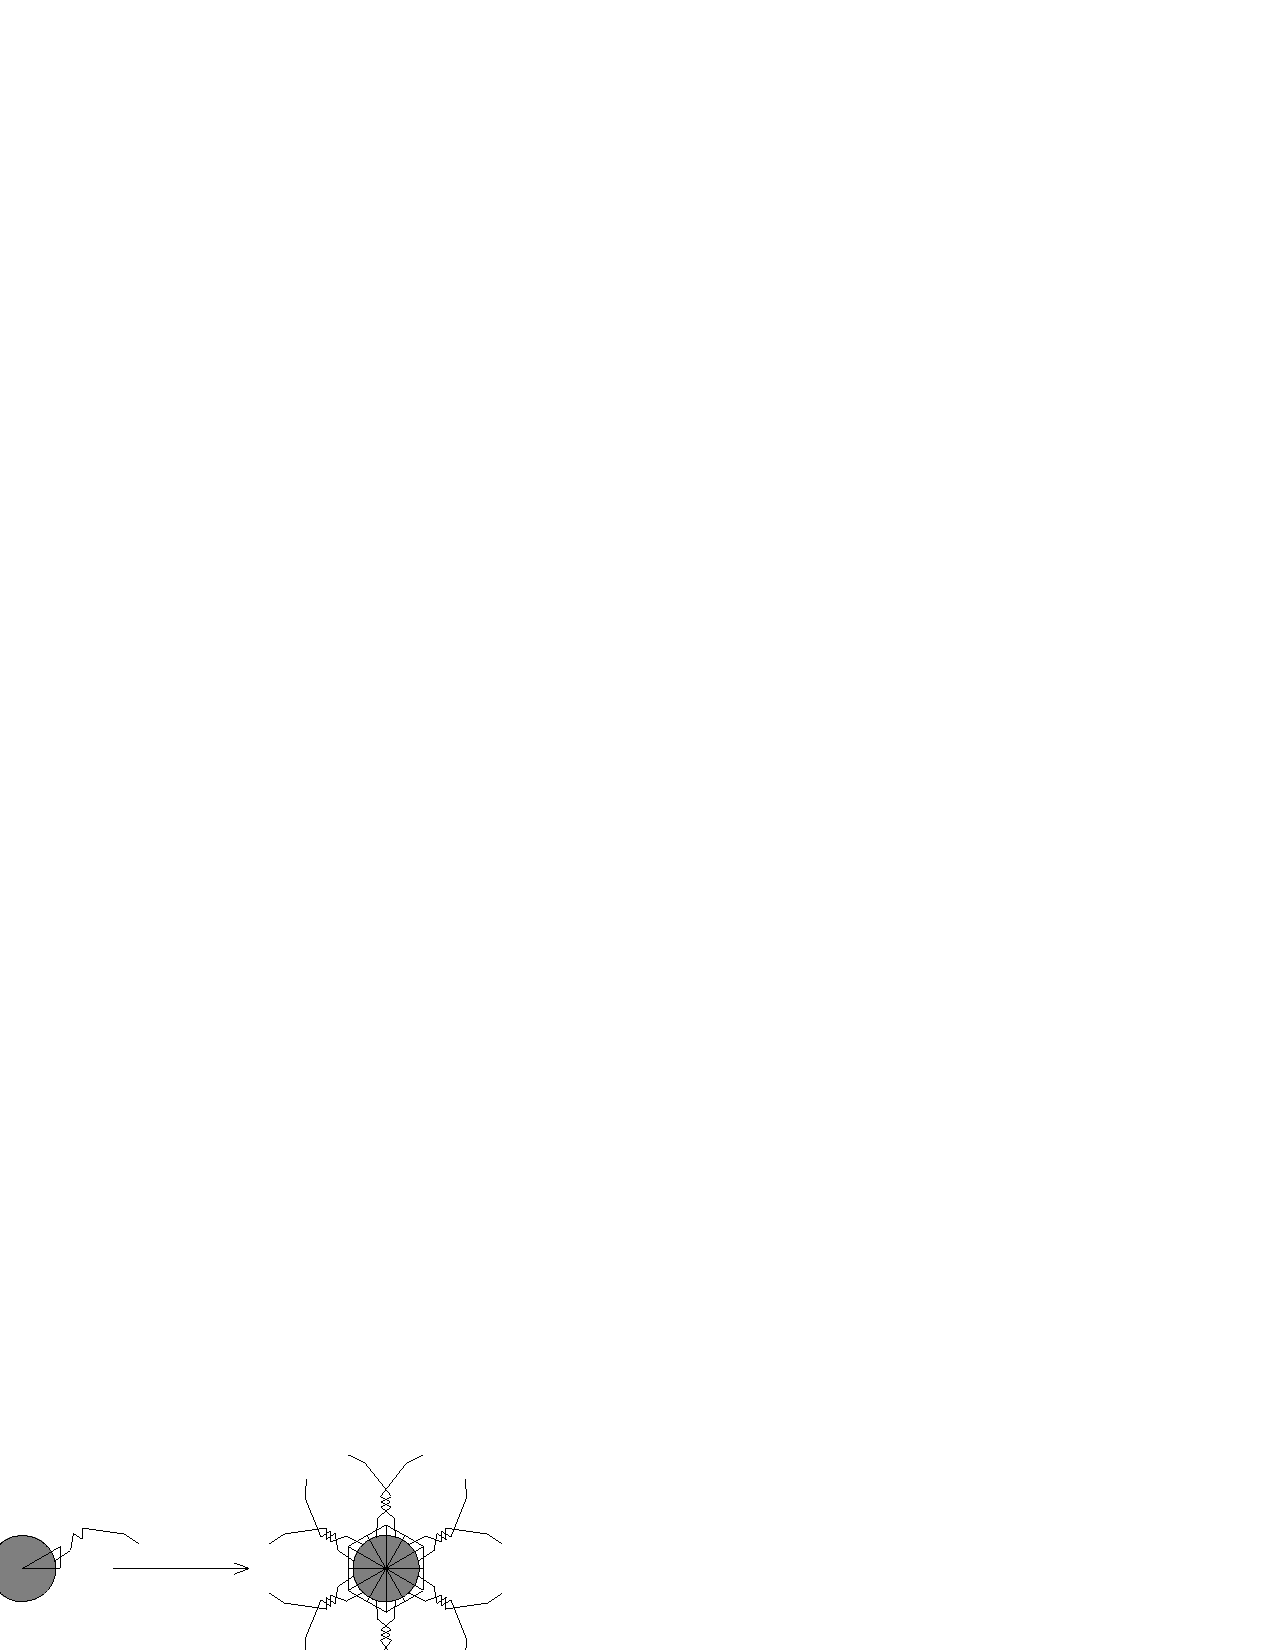
\includegraphics[width=0.45\textwidth]{schreiberFig2}
\end{center}
\caption{
$\hp $ is the discrete transformation that relates the endpoint
of the cycle $\tp \in \tM$ to the endpoint of the corresponding
trajectory segment in $M$.
Eckmann\rf{LorentzDiff} Fig.~2. Remember to include
schreiberFig2.tex
    }
\label{schreiberFig2}
\end{figure}
%%%%%%%%%%%%%%%%%%%%%%%%%%%%%%%%%%%%%%%%%%%%%%%%%%%%%%%%%%%%%%%%%%%%%%%%



\section{Figure captions}

%%%%%%%%%%%%%%\item[Figure 1]%%%%%%%%%%%%%%%%%%%%%%%%%%%%%%%%%%%%%%%%%%
\begin{figure}
\begin{center}
\setlength{\unitlength}{25pt} \begin{picture}(3,3)(1.5,1.5)
\put(5.15,3.336){\line(0,1){1.336}} \put(2.85,3.336){\line(0,1){1.336}}
\put(4,2.646){\line(5,3){1.15}}     \put(4,2.646){\line(-5,3){1.15}}
\put(4,5.354){\line(5,-3){1.15}}    \put(4,5.354){\line(-5,-3){1.15}}
\put(4,4){\line(5,3){1.15}}         \put(4,4){\line(1,0){1.15}}
\put(4,4){\circle{2}}        \put(6.3,4){\circle{2}} \put(1.7,4){\circle{2}}
\put(5.15,5.992){\circle{2}} \put(2.85,5.992){\circle{2}}
\put(5.15,2.008){\circle{2}} \put(2.85,2.008){\circle{2}}
\put(2.85,2.008){\line(0,-1){0.7}} \put(2.85,0.7){\line(0,1){0.4}}
\put(3.65,1.9){\line(0,-1){1.2}}   \put(4.35,1.9){\line(0,-1){1.2}}
\put(3,0.8){\vector(-1,0){0.15}}   \put(2.85,0.8){\vector(1,0){0.8}}
\put(4,0.8){\vector(-1,0){0.35}}   \put(4,0.8){\vector(1,0){0.35}}
\put(3.8,0.4){$w$} \put(3.1,0.4){1}
\end{picture}
\end{center}
\caption{
 A small portion of a triangular Lorentz gas. The whole set of scatterers
can be obtained by translating  the
%hexagonal
elementary cell indicated in the figure.
%The arrangement can also be tiled with images of the fundamental domain
%under the symmetry group of the hexagon.
    }
\label{schreiberFig0}
\end{figure}
%%%%%%%%%%%%%%%%%%%%%%%%%%%%%%%%%%%%%%%%%%%%%%%%%%%%%%%%%%%%%%%%%%%%%%%%

\begin{description}

\item[Figure 2]
 A portion of a chaotic trajectory with about 300 bounces is shown.
Although the particle is often trapped between neighboring disks
%one of the triangular enclosures
for several bounces, there are also
segment of the trajectory
which take the particle over a large distance with few bounces.

\item[Figure 3]
The upper row shows the case when the preceding
segment has been a long one,
the lower row the case when it has been a short one.
The arrows at the end points
indicate the sense of the next change of direction.
Due to the discrete symmetry of the triangular lattice,
all translated, rotated or reflected copies of each
situation shown are denoted by the same symbol.

\item[Figure 4]
The upper row shows the case when the preceding
segment has been a short one,
the lower row the case when it has been a long one.

 \item[Figure 5]
Shown are global orbits which reduce to fixed points in the fundamental
domain. Five of them (a,b,c,C,D) are not pruned for $w=0.3$,
the spacing shown here. The sixth (B) is an example of a pruned
cycle; it exists for a dilute Lorentz gas, because
for the dense Lorentz gas its trajectory is blocked by the center
disk. Both B and D denote turns by 120 degrees, but
D also changes the sense of rotation at each bounce.
\end{description}

%%%%%%%%%%%%%%\item[Figure 2]%%%%%%%%%%%%%%%%%%%%%%%%%%%%%%%%%%%%%%%%%%
\begin{figure}
\begin{center}
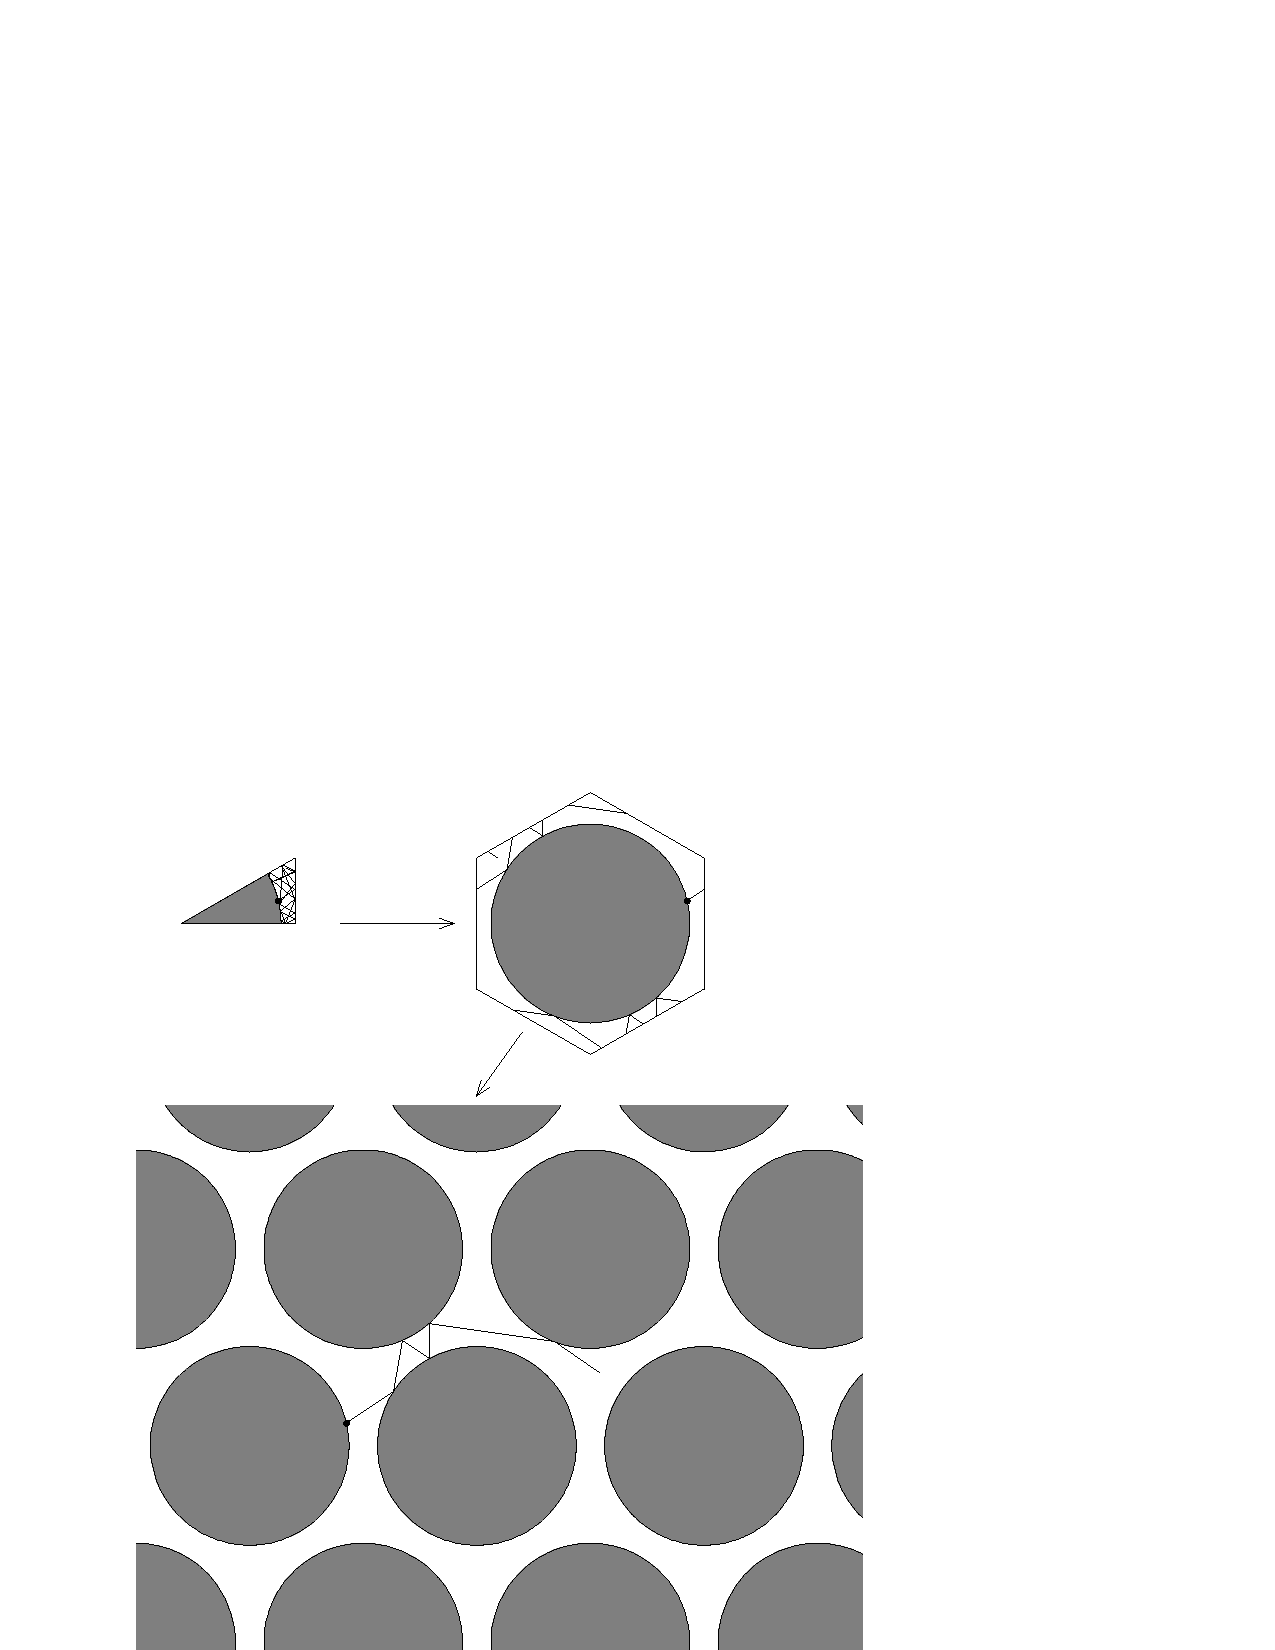
\includegraphics[width=0.45\textwidth]{schreiberFig1}
\end{center}
\caption{
Eckmann\rf{LorentzDiff} Fig.~1, from dif15.pdf. Remember to include
(misnamed) schreiberFig1.tex
    }
\label{schreiberFig1}
\end{figure}
%%%%%%%%%%%%%%%%%%%%%%%%%%%%%%%%%%%%%%%%%%%%%%%%%%%%%%%%%%%%%%%%%%%%%%%%

%%%%%%%%%%%%%%\item[Figure 4]%%%%%%%%%%%%%%%%%%%%%%%%%%%%%%%%%%%%%%%%%%
\begin{figure}
\begin{center}
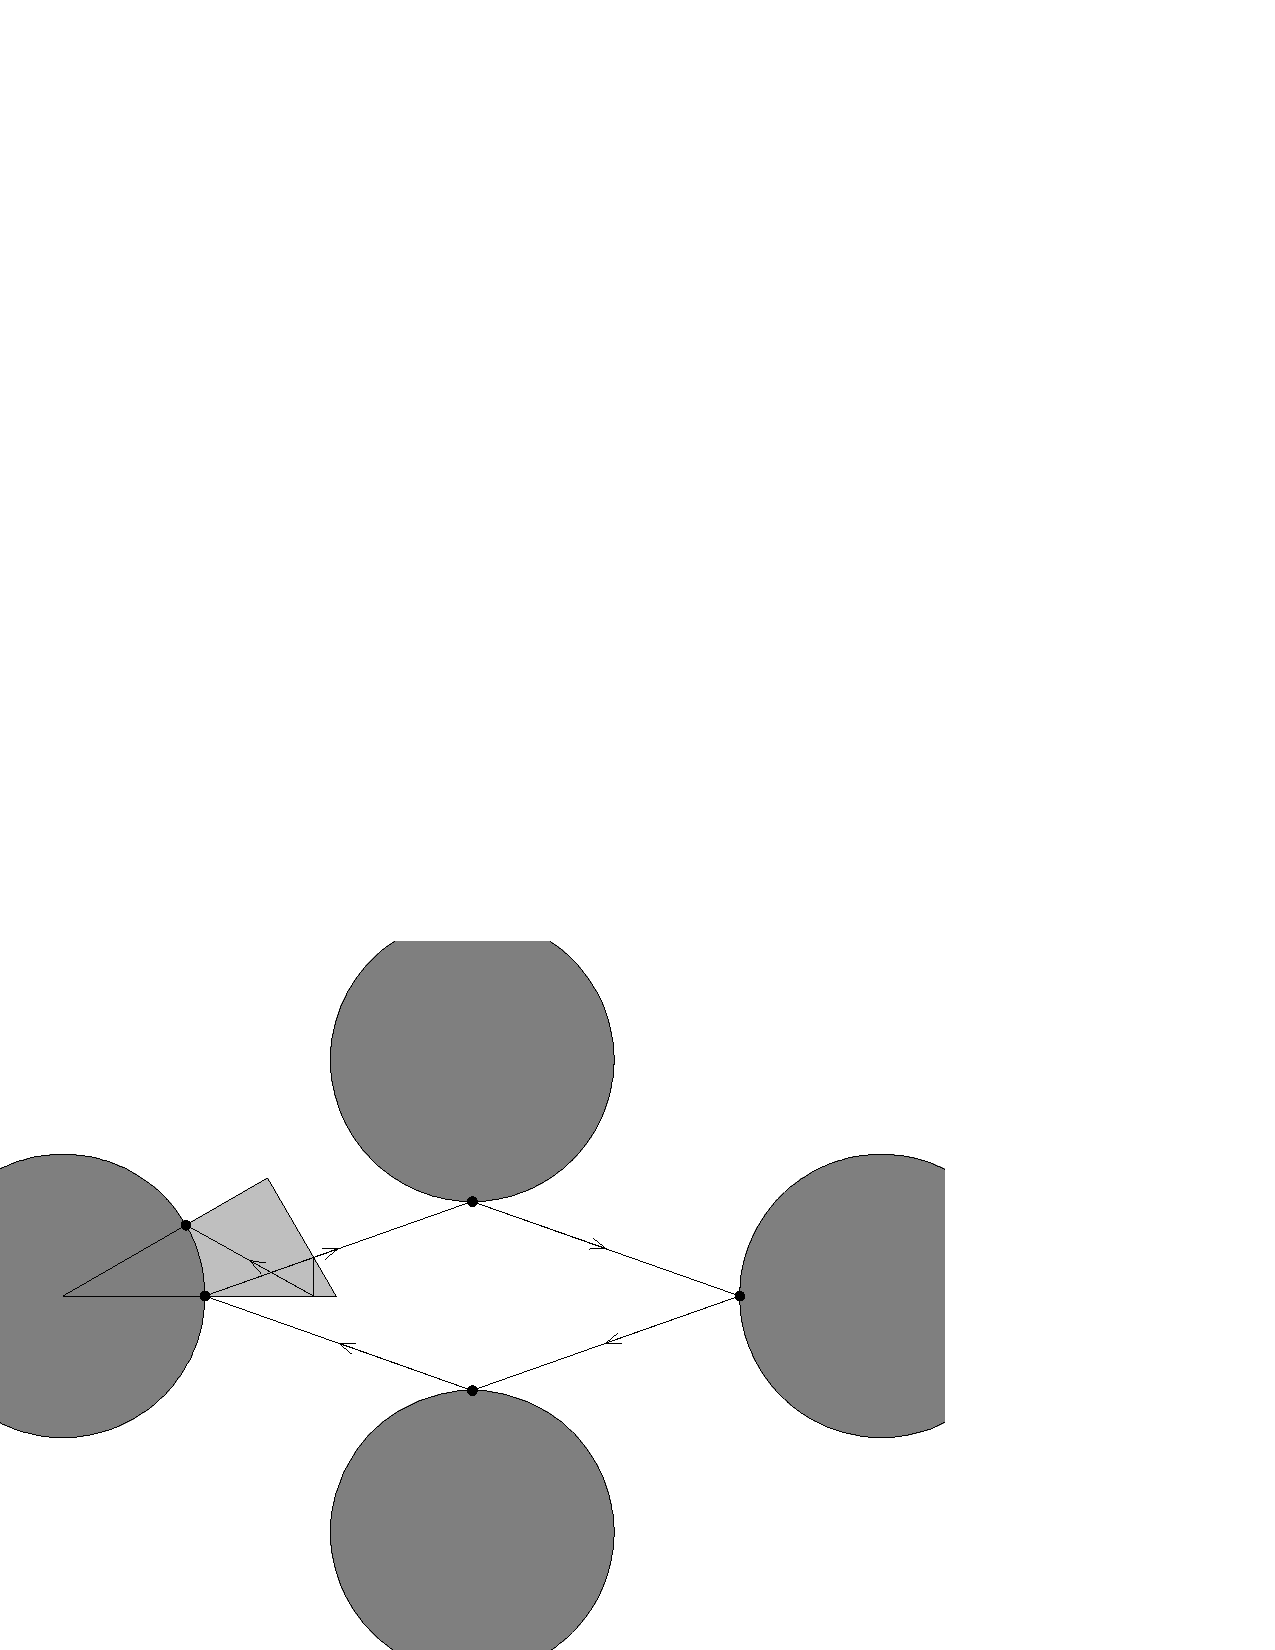
\includegraphics[width=0.45\textwidth]{schreiberFig3}
\end{center}
\caption{
Eckmann\rf{LorentzDiff} Fig.~3. Remember to include
schreiberFig3.tex
    }
\label{schreiberFig3}
\end{figure}
%%%%%%%%%%%%%%%%%%%%%%%%%%%%%%%%%%%%%%%%%%%%%%%%%%%%%%%%%%%%%%%%%%%%%%%%




%%%%%%%%%%%%%%%%%%%%%%%%%%%%%%%%%%%%%%%%%%%%%%%%%%%%%%%%%%%%%

\newpage
\bibliographystyle{../inputs/adkPCphysrev} % PC trying Phys Rev style,
                                            % but with article titles
					   % ES: this exists as an option in revtex 4.1
					    % use [longbibliography] in class options
% \bibliographystyle{../inputs/siam}
% \bibliographystyle{../inputs/apsrev} % PC playing with bib styles...
% \bibliographystyle{plain}
\addcontentsline{toc}{chapter}{Bibliography}
\bibliography{../bibtex/siminos}

\newpage
\section{Daily blog}
\label{sect-DailyBlog}

\begin{description}

\item[2013-02-03 Roberto]
incorporate kneading determinants from
G.~Cristadoro\rf{Cristad06}
{\em Fractal diffusion coefficient from dynamical zeta functions}.

\item[2009-02-27 Predrag]
Read  Gilbert  and Lefevere\rf{GilbLef08},
    ``Heat conductivity from molecular chaos hypothesis
             in locally confined billiard systems,''

``From Deterministic Chaos to Deterministic Diffusion''
by R. Klages, \arXiv{0804.3068}: ``
A set of easy-to-read lecture notes for a short first-year Ph.D.
student course. The notes cover five hours of lectures and
do not require any prior knowledge on dynamical systems. The first part introduces
to deterministic chaos in one-dimensional maps in form of Lyapunov exponents
and the metric entropy. The second part first outlines the concept of
deterministic diffusion. Then the escape rate formalism for deterministic
diffusion, which expresses the diffusion coefficient in terms of the above two
chaos quantities, is worked out for a simple map. The notes conclude with a
very brief sketch of anomalous diffusion.

For `fundamental domain' in hyperbolic geometry, see for example
\HREF{http://www.math.ou.edu/~kmartin/mfs/ch3.pdf}{these notes}
by \HREF{http://www.math.ou.edu/~kmartin}{Kimball Martin}.

\item[2014-02-27 Predrag] Must read:
Dettmann\rf{Dettm14}, {\em Diffusion in the {Lorentz} gas}.

generate \texttt{f\_diff\_MarkPart.pdf}
from \texttt{.../xfig/f\_diff\_MarkPart.fig}

\item[2013-02-28 Predrag] to Tingnan Zhang:
Dettmann's review, \arXiv{1402.7010} is something that you want to read -
looks very complete. {\bf Goldman:} Sects. 7.4 and 7.5 and refs within
are tantalizing.

\item[2013-03-25 Predrag] to Tingnan Zhang:
{\em Superdiffusion in the periodic Lorentz gas} by
Jens Marklof and Balint Toth,  	\arXiv{1403.6024} is too mathematical and
general for our purposes (hopefully we will have no super-diffusivity, noise
should wipe that out), but
Sect.~2~{\em The scattering map} might be useful for your exposition
(or its prequel  \arXiv{0801.0612}).

\item[2014-04-18 Predrag]
Sinai\rf{Sinai04} might be a quick read.
Recent references of possible interest:
Zhang\rf{HKZhang11}
{\em Current in periodic {Lorentz} gases with twists}.

\item[2014-04-18 Predrag]
I have saved the Lorentz\rf{Lorentz1905} 1905
{\em The motion of electrons in metallic bodies}
(\HREF{http://chaosbook.org/library/index.html}{click here}).

\end{description}


\end{document}
